\documentclass[10pt]{memoir}
\setstocksize{220mm}{155mm} 	        
\settrimmedsize{220mm}{155mm}{*}	
\settypeblocksize{170mm}{116mm}{*}	
\setlrmargins{18mm}{*}{*}
\setulmargins{*}{*}{1.2}
%\setlength{\headheight}{5pt}%
\checkandfixthelayout[lines]
\linespread{1.16}
\flushbottom

%%% Hyphenation settings
\usepackage[htt]{hyphenat}
\hyphenation{he-lio-trope opos-sum}
\tracingparagraphs=1
%Hyphenation in Devanāgarī of the edition still missing? Probably this needs to be modified in babel-iast package? 

%%% babel
\usepackage[english]{babel}
\usepackage{babel-iast/babel-iast}

\babelfont[iast]{rm}[Renderer=Harfbuzz, Scale=1.3]{AdishilaSan}%AdishilaSan}
\babelfont[english]{rm}{Adobe Text Pro}

%%% more functionality
\PassOptionsToPackage{hyphens}{url}
\usepackage{hyperref}
\usepackage{pdflscape}
\usepackage{cleveref}
\usepackage{url}
\usepackage{cleveref}
\usepackage{microtype}
\usepackage{lineno}

%\usepackage{bigfoot}
%%% more functions
\usepackage[dvipsnames]{xcolor}
%\usepackage[para,perpage]{footmisc}

%%%für den Counter von Kapiteln und Sätzen! 
\newcommand{\uproman}[1]{\uppercase\expandafter{\romannumeral#1}}
\newcommand{\lowroman}[1]{\romannumeral#1\relax}

\makeindex
\newfontfamily\sanskritfont[Script=Devanagari,Mapping=RomDev,Scale=1.1]{Sanskrit2003}
\usepackage{pifont,fourier-orns,lettrine,psvectorian,paralist,enumitem,pdfpages,wrapfig,tabulary,lettrine,longtable}
\setlist[enumerate]{itemsep=0mm}
\usepackage[autostyle]{csquotes}
\usepackage[defaultlines=2,all]{nowidow}
\usepackage{ellipsis,adforn,booktabs,longtable,url,tikz}
\lineskiplimit=-3pt          

\makechapterstyle{IeT}{%
  \chapterstyle{default}
  \renewcommand*{\printchapternonum}{\centering}
  \renewcommand*{\clearforchapter}{\cleartorecto} 
  \aliaspagestyle{chapter}{empty}}
\chapterstyle{IeT}
\setsecnumdepth{none}  \openright  \nouppercaseheads
\settocdepth{subsubsection}

%%%% test better pagebreaks
%\def\fussy{%
%  \emergencystretch\z@
%  \tolerance 200%
%  \hfuzz .1\p@
%  \vfuzz\hfuzz}

%\interfootnotelinepenalty=10000\relax

%\usepackage[maxfloats=256]{morefloats}

%\maxdeadcycles=500

%raggedbottomsectiontrue
%%\checkandfixthelayout


%%%%%%%  biblatex
%\newcommand{\noun}[1]{\textsc{#1}}    %  philosophy-verbose
\usepackage[backend=biber, sorting=nyt, style=verbose]{biblatex} %%%%ORIGINAL TiE
\renewcommand*{\mkbibnamefamily}[1]{\textsc{#1}}


\DeclareFieldFormat{url}{%
  \mkbibacro{URL}\addcolon\space
  \href{#1}{\nolinkurl{\thefield{urlraw}}}}

\DeclareFieldFormat{citeurl}{%
  \href{#1}{\nolinkurl{\thefield{urlraw}}}} 


\DeclareFieldFormat{postnote}{#1}
\renewcommand{\postnotedelim}{, }
\addbibresource{bindu.bib}

%%% ekdosis
\usepackage[teiexport=tidy,parnotes=true]{ekdosis}% =tidy cleans up HTML and XML documents by fixing markup errors and upgrading legacy code to modern standards. parnotes=footnotes below or above critical apparatus

\SetLineation{lineation=page, modulo} %lineation=page sets thenumbering to start afresh at the top of each page. =modulo makes every fifth line numbered. {lineation=page} makes every line numbered! 

\renewcommand{\linenumberfont}{\selectlanguage{english}\footnotesize} %sets language of lines to English

\SetTEIxmlExport{autopar=false} %autopar=falseinstructs ekdosis to ignore blank lines in the.tex sourcefile as markers for paragraph boundaries. As a result, each paragraph of the edition must be found within an environment associated with the xml <p> element

\SetHooks{
  lemmastyle=\bfseries,
  %refnumstyle=\selectlanguage{english}\bfseries,
  refnumstyle=\selectlanguage{english}\color{blue}\bfseries,
  appheight=0.8\textheight,
}

\newif\ifinapparatus
\DeclareApparatus{source}[
%bhook=\inapparatustrue,
lang=english,
notelang=english,
% bhook=\selectlanguage{english},
bhook=\selectlanguage{english}\textbf{Sources:},%
%maxentries=4, 
%ehook=.]
%sep={] },
%nosep,
]

\newif\ifinapparatus
\DeclareApparatus{testium}[
%bhook=\inapparatustrue,
lang=english,
notelang=english,
% bhook=\selectlanguage{english},
bhook=\selectlanguage{english}\textbf{Testimonia:},
%maxentries=4, 
%ehook=.]
%nosep, 
]

% Declare \ifinapparatus and set \inapparatustrue at the beginning of
% the apparatus criticus block. Also set the language.  
\newif\ifinapparatus
  \DeclareApparatus{default}[
  %bhook=\inapparatustrue, 
  lang=english,
  %maxentries=33,
  %bhook=\selectlanguage{english},
  sep = {] },
  delim=\hskip 0.75em,
  rule=\rule{0.7in}{0.4pt},
]

\newif\ifinapparatus
\DeclareApparatus{philcomm}[
%bhook=\inapparatustrue,
lang=english,
notelang=english,
bhook=\selectlanguage{english}\textbf{Philological Commentary:},
%bhook=\selectlanguage{english},
sep={: },
]

\ekdsetup{
showpagebreaks,
spbmk = \textcolor{blue}{spb},
hpbmk = \textcolor{red}{hpb}
}

%\usepackage{fnpos}
%\makeFNmid
%\makeFNbottom
\usepackage[bottom]{footmisc}
%%%%%%%%%%%%%%%%%%%%%%%%%%%
\makeatletter
\def\blfootnote{\gdef\@thefnmark{}\@footnotetext}
\makeatother
%%%%%%%%%%%%%%%%%%%%%%%%%


% Macros and Definitions for the Print of Sigla
\def\acpc#1#2#3{{#1}\rlap{\textrm{\textsuperscript{#3}}}\textsubscript{\textrm{#2}}\space}
\def\sigl#1#2{{{#1}}\textsubscript{\textrm{#2}}}
\def\None{{\sigl{N}{1}}} \def\Noneac{\acpc{N}{1}{ac}\,} \def\Nonepc{\acpc{N}{1}{pc}\,}
\def\Ntwo{{\sigl{N}{2}}} \def\Noneac{\acpc{N}{2}{ac}\,} \def\Nonepc{\acpc{N}{2}{pc}\,}
\def\Done{{\sigl{D}{1}}} \def\Doneac{\acpc{D}{1}{ac}\,} \def\Donepc{\acpc{D}{1}{pc}\,}
\def\Dtwo{{\sigl{D}{2}}} \def\Dtwoac{\acpc{D}{2}{ac}\,} \def\Dtwopc{\acpc{D}{2}{pc}\,}
\def\Uone{{\sigl{U}{1}}} \def\Uoneac{\acpc{U}{1}{ac}\,} \def\Uonepc{\acpc{U}{1}{pc}\,}                 
\def\Utwo{{\sigl{U}{2}}} \def\Utwoac{\acpc{U}{2}{ac}\,} \def\Utwopc{\acpc{U}{2}{pc}\,}

%%%%%%%%%%%%%% Tattvabinduyoga - List of Witnesses   %%%%%%%%%%%%%%%%%%%
\DeclareWitness{ceteri}{\selectlanguage{english}cett.}{ceteri}[]   
\DeclareWitness{E}{\selectlanguage{english}E}{Printed Edition}[]    
\DeclareWitness{P}{\selectlanguage{english}P}{Pune BORI 664}[]  
\DeclareWitness{B}{\selectlanguage{english}B}{Bodleian 485}[]       
\DeclareWitness{N1}{\selectlanguage{english}N\textsubscript{1}}{NGMPP 38/31}[]
\DeclareWitness{N2}{\selectlanguage{english}N\textsubscript{2}}{NGMPP B 38/35}[]
\DeclareWitness{L}{\selectlanguage{english}L}{LALCHAND 5876}[]  
\DeclareWitness{D}{\selectlanguage{english}D}{IGNCA 30019}[] 
%\DeclareWitness{D2}{\selectlanguage{english}D\textsubscript{2}}{IGNCA 30020}[]  
\DeclareWitness{U1}{\selectlanguage{english}U\textsubscript{1}}{SORI 1574}[] 
\DeclareWitness{U2}{\selectlanguage{english}U\textsubscript{2}}{SORI 6082}[]
%%%%%%%%%%%%%% Tattvabinduyoga - Groups of Witnesses   %%%%%%%%%%%%%%%%%%%
\DeclareWitness{X}{\selectlanguage{english}\alpha}{Alpha Group: D,N1,N2,U1}[]
\DeclareWitness{Y}{\selectlanguage{english}\beta}{Beta Group: B,E,L,P,U2}[]
%%%%%%%%%%%%% Testimonia
\DeclareWitness{Ysv}{\selectlanguage{english}Ysv}{Yogasvarodaya}[] %%%add infos!  

%%%%%%%%%%%%%%%%%%%%%%%%%%%%%%%%%%%%%%%%%%%
% Macro for Editing Abbrevs.
\def\om{\textrm{\footnotesize \textit{om.}\ }} %prints om. for omitted in apparatus
\def\korr{\textrm{\footnotesize \textit{em.}\ }} %prints em. for emended in apparatus
\def\conj{\textrm{\footnotesize \textit{conj.}\ }} %prints conj. for conjectured in apparatus

% \supplied{text} EDITORIAL ADDITION -> Within \lem oder \rdg
% \surplus{text} EDITORIAL DELETION -> Within \lem oder \rdg
% \sic{text} CRUX
% \gap{text} LACUNAE -> [reason=??, unit=??, quantity=??, extent=??]


%%%%%%%%%%%%%%%%%%%%%%%%%%%%%%%%%%%%%%%%%%% All macros of this list can be used in 
% Macro for Editing Abbrevs.
\def\eyeskip{\textrm{{ab.\,oc. }}}
\def\aberratio{\textrm{{ab.\,oc. }}}
\def\ad{\textrm{{ad}}}
\def\add{\textrm{{add.\ }}}
\def\ann{\textrm{{ann.\ }}}
\def\ante{\textrm{{ante }}} 
\def\post{\textrm{{post }}}
%\def\ceteri{cett.\,}                   
\def\codd{\textrm{{codd.\ }}}

\def\coni{\textrm{{coni.\ }}}
\def\contin{\textrm{{contin.\ }}}
\def\corr{\textrm{{corr.\ }}}
\def\del{\textrm{{del.\ }}}
\def\dub{\textrm{{ dub.\ }}}

\def\expl{\textrm{{explic.\ }}} 
\def\explica t{\textrm{{explic.\ }}}
\def\fol{\textrm{{fol.\ }}}
\def\foll{\textrm{{foll.\ }}}
\def\gloss{\textrm{{glossa ad }}}
\def\ins{\textrm{{ins.\ }}}      
\def\inseruit{\textrm{{ins.\ }}} 
\def\im{{\kern-.7pt\lower-1ex\hbox{\textrm{\tiny{\emph{i.m.}}}\kern0pt}}} %\textrm{\scriptsize{i.m.\ }}}      
\def\inmargine{{\kern-.7pt\lower-.7ex\hbox{\textrm{\tiny{\emph{i.m.}}}\kern0pt}}}%\textrm{\scriptsize{i.m.\ }}}      
\def\intextu{{\kern-.7pt\lower-.95ex\hbox{\textrm{\tiny{\emph{i.t.}}}\kern0pt}}}%\textrm{\scriptsize{i.t.\ }}}           
\def\indist{\textrm{{indis.\ }}}  
\def\indis{\textrm{{indis.\ }}}
\def\iteravit{\textrm{{iter.\ }}} 
\def\iter{\textrm{{iter.\ }}}
\def\lectio{\textrm{{lect.\ }}}   
\def\lec{\textrm{{lect.\ }}}
\def\leginequit{\textrm{{l.n. }}} 
\def\legn{\textrm{{l.n. }}}
\def\illeg{\textrm{{l.n. }}}

\def\primman{\textrm{{pr.m.}}}
\def\prob{\textrm{{prob.}}}
\def\rep{\textrm{{repetitio }}}
\def\secundamanu{\textrm{\scriptsize{s.m.}}}            \def\secm{{\kern-.6pt\lower-.91ex\hbox{\textrm{\tiny{\emph{s.m.}}}\kern0pt}}}%   \textrm{\scriptsize{s.m.}}}
\def\sequentia{\textrm{{seq.\,inv.\ }}}  
\def\seqinv{\textrm{{seq.\,inv.\ }}}
\def\order{\textrm{{seq.\,inv.\ }}}
\def\supralineam{{\kern-.7pt\lower-.91ex\hbox{\textrm{\tiny{\emph{s.l.}}}\kern0pt}}} %\textrm{\scriptsize{s.l.}}}
\def\interlineam{{\kern-.7pt\lower-.91ex\hbox{\textrm{\tiny{\emph{s.l.}}}\kern0pt}}}   %\textrm{\scriptsize{s.l.}}}
\def\vl{\textrm{v.l.}}   \def\varlec{\textrm{v.l.}} \def\varialectio{\textrm{v.l.}}
\def\vide{\textrm{{cf.\ }}}
\def\cf{\textrm{{cf.\ }}} 
\def\videtur{\textrm{{vid.\,ut}}}
\def\crux{\textup{[\ldots]} }
\def\cruxx{\textup{[\ldots]}}
\def\unm{\textit{unm.}}
%%%%%%%%%%%%%%%%%%%%%%%%%%%%%%%%%%%%

% List of Scholars
\DeclareScholar{ego}{ego}[
forename=Nils Jacob,
surname=Liersch]

% Persons:14\DeclareScholar{ego}{ego}[15forename=Robert,16surname=Alessi]17% Useful shorthands:18\DeclareShorthand{codd}{codd.}{V,I,R,H}19\DeclareShorthand{edd}{edd.}{Lit,Erm,Sm}20\DeclareShorthand{egoscr}{\emph{scripsi}}{ego}

%Useful shorthands:
%\DeclareShorthand{codd}{codd.}{V,I,R,H}
%\DeclareShorthand{edd}{edd.}{Lit,Erm,Sm}
\DeclareShorthand{egoscr}{em.}{ego}
\DeclareShorthand{egoscrconj}{conj.}{ego}
\DeclareShorthand{egomute}{\unskip}{ego}

\usepackage{xparse}

\NewDocumentEnvironment{tlg}{O{}O{}}{\setlength{\leftskip}{0pt}\vspace{-1ex}\begin{quotation}}{\hfill #1\ \vspace{-1ex}\end{quotation}\vspace{-1ex}} %verse environment
%\NewDocumentEnvironment{tlg}{O{}O{}}{\begin{verse}}{॥#1\hskip-4pt ॥\\ \end{verse}}
\NewDocumentCommand{\tl}{m}{{\selectlanguage{iast} #1}}

\NewDocumentCommand{\extra}{m}{{\textcolor{gray}{#1}}} %command for additions to U2
\NewDocumentCommand{\crazy}{m}{{\textcolor{red}{#1}}} %totally corrupted passage
\NewDocumentCommand{\coro}{m}{{\textcolor{violet}{#1}}} %colour for sentence counter! 

\NewDocumentEnvironment{prose}{O{}}{\begin{otherlanguage}{iast}}{\end{otherlanguage}}
% \NewDocumentEnvironment{padd}{O{}}{\begin{otherlanguage}{iast}}{\end{otherlanguage}}
\NewDocumentEnvironment{tlate}{O{}}
%\NewDocumentEnvironment{tadd}{O{}}

%Define two commands: \skp ("sanskrit plus"), to be ignored by TeX in
%the edition text, but processed in the TEI output. Conversely, \skm
%("sanskrit minus") is to be processed in the edition text, but
%ignored if found in the apparatus criticus and in the TEI output:

\NewDocumentCommand{\skp}{m}{}
\TeXtoTEIPat{\skp {#1}}{#1}

%\NewDocumentCommand{\skpp}{m}{}
%\TeXtoTEIPat{\skpp {#1}}{#1}

\NewDocumentCommand{\skm}{m}{\unless\ifinapparatus#1-\fi}
\TeXtoTEIPat{\skm {#1}}{}

% \NewDocumentCommand{\dd}{}{/\hskip-4pt/}
\NewDocumentCommand{\dd}{}{\mbox{/\hskip-4pt/}}
\TeXtoTEIPat{\dd {}}{//}


%%% modify environments and commands
%%% TEI mapping
\TeXtoTEIPat{\begin {tlg}}{<lg>} %lg=(Group of verse (s)) contains one or more verses or lines of verse that together form a formal unit (e.g. stanza, chorus).
\TeXtoTEIPat{\end {tlg}}{</lg>}

\TeXtoTEIPat{\begin {prose}}{<p>}
\TeXtoTEIPat{\end {prose}}{</p>}

\TeXtoTEIPat{\begin {tlate}}{<p>}
\TeXtoTEIPat{\end {tlate}}{</p>}

\TeXtoTEIPat{\\}{}
\TeXtoTEIPat{\linebreak}{<br/>}
\TeXtoTEIPat{\noindent}{}
%\TeXtoTEI{tl}{l}
\TeXtoTEI{emph}{hi}
\TeXtoTEI{bigskip}{}
\TeXtoTEI{None}{N1}
\TeXtoTEI{Ntwo}{N2}
\TeXtoTEI{Done}{D1}
\TeXtoTEI{Dtwo}{D2}
\TeXtoTEI{Uone}{U1}
\TeXtoTEI{Utwo}{U2}
%\TeXtoTEIPat{/}{ |}
%\TeXtoTEI{//}{ ||}
\TeXtoTEIPat{\korr}{em. }
\TeXtoTEIPat{\conj}{conj.}
\TeXtoTEIPat{\om}{om.}
\TeXtoTEIPat{english}{}
\TeXtoTEIPat{\hskip}{}
\TeXtoTEIPat{\hskip-4pt}{}
\TeXtoTEIPat{\hskip-2pt}{}
\TeXtoTEIPat{-}{ }
\TeXtoTEIPat{4pt}{}
\TeXtoTEIPat{2pt}{}
\TeXtoTEIPat{\textcolor {#1}{#2}}{<hi rend="#1">#2</hi>} 

% Nullify \selectlanguage in TEI as it has been used in
% \DeclareWitness but should be ignored in TEI.
\TeXtoTEI{selectlanguage}{}



\FormatDiv{1}{\begin{center}\Large}{\end{center}}
\FormatDiv{2}{\begin{center}\small}{\end{center}}
\FormatDiv{3}{\bfseries}{.}
\title{Yogatattvabindu of Rāmacandra\\ A Critical Edition and Annotated Translation}
\date{\today}

\parindent=15pt
\begin{document}

% Zitiermöglichkeiten:
%\footcite[See][p.\,1]{goldstein01:_tibet_englis_diction_moder_tibet}
%\footnote{\cite{goldstein01:_tibet_englis_diction_moder_tibet}.}

\frontmatter
\thispagestyle{empty}
\begin{center}
  {\Large \emph{The Yogatattvabindu}}\\[3mm]
\end{center}



\newpage

\

\thispagestyle{empty}



\normalsize


\newpage


\begin{center}
\thispagestyle{empty}

\

\vskip 2mm

\begin{otherlanguage}{iast}
\LARGE \sanskritfont{Yogatattvabindu}
\end{otherlanguage}

\vskip .4cm

\Huge Yogatattvabindu \\[7mm]
\Large Critical Edition\\
with annotated Translation


\large

\vspace{3cm}

Von

Nils Jacob Liersch
\small
\vfill

\vfill

Indica et Tibetica Verlag \\ % $\cdot$ 
Marburg 2024

\vskip 6mm

\end{center}

\newpage
\newpage \ \thispagestyle{empty}
\small  \

\noindent

\
\vfill


\small
\noindent \textbf{Bibliographische Information Der Deutschen Bibliothek}

\noindent
Die Deutsche Bibliothek verzeichnet diese Publikation in der Deutschen Nationalbibliographie;
detaillierte bibliographische Informationen sind im Internet über http://dnb.ddb.de abrufbar.

\noindent
\textbf{Bibliographic information published by Die Deutschen Bibliothek}

\noindent
Die Deutsche Bibliothek lists this publication in the Deutsche Nationalbibliographie; detailed
bibliographic data is available in the Internet at http://dnb.ddb.de.  


\vskip 1cm

\noindent
\copyright\ Indica et Tibetica Verlag, Marburg 2024

\medskip

\noindent
Alle Rechte vorbehalten / All rights reserved

\medskip

\noindent
Ohne ausdrückliche Genehmigung des Verlages ist es nicht gestattet, das Werk oder einzelne Teile
daraus nachzudrucken, zu vervielfältigen oder auf Datenträger zu speichern.

\smallskip

\noindent
Apart from any fair dealing for the purpose of private study, research, criticism or review, no
part of this book may be reproduced or translated in any form, by print, photo form, microfilm, or
any other means without written permission. Enquiries should be made to the publishers.

\bigskip

\noindent
Satz: \ \ Nils Jacob Liersch \\
Herstellung: \ \ BoD – Books on Demand GmbH, Norderstedt  \\

\bigskip

\noindent
%\ISBN     

\normalsize

\newpage

%\maketitle
\clearpage
\tableofcontents
\addtocounter{page}{-1}
\thispagestyle{empty}
\clearpage


\mainmatter

\chapter{Conventions in the Critical Apparatus}
\section{Sigla in the Critical Apparatus}

\begin{itemize}
\item E : Printed Edition
\item P : Pune BORI 664
\item L : Lalchand Research Library LRL5876
\item B : Bodleian Oxford D 4587
\item \None : NGMPP B 38-31
\item \Ntwo : NGMPP B 38-35 / A 1327-14
\item \Done : IGNCA 30019
\item \Uone : SORI 1574
\item \Utwo: SORI 6082
\end{itemize}

\chapter{Critical Edition \& Annotated Translation}
\cleardoublepage
\begin{alignment}[
  texts=edition[class="edition"];
  translation[class="translation"],
  ]
  \begin{edition}
    \ekddiv{type=ed}
    \begin{tlg}
      \noindent
  \note[type=source, labelb=418, nosep]{cf. YSv (PT p. 847): idaṃ yogarahasyañ ca na vācyaṃ mūrkhasannidhau || yogadeśas tu tatraiva ||}
%-----------------------------
%na snehān na bhayān na lobhān na mohān na dhanād   balān    na maitrībhāvān  nau dāryān na sauṃdaryān na sevanāt/ \E
%na snehān no bhayāl lno?                                             bhāvān  no  dānān  na sau daryān na sevanāt  \P %%%7680.jpg
%ni śnehān nā bhayāl lobhān    na mohān na dhanād   balāt/   na maitrībhāvān  no  dānāt  na sauṃdaryān na sevanāt/ \B
%ni śnehān nā bhayāl lobhān    na mohān na nadhanād balāta// na maitrībhāvān  no  dānāt  na sauṃdayan  ni sevanāt// \L
%na śnehān a  bhayāl obhān     na mohān na dhanād   balāt/   na maitrībhāvān  na  dāsān  na sauṃdaryān na sevanāt/ \N1
%na śnehān a  bhayāl obhān     na mohān na dhanād   balāt//  na maitrībhāva   nā  dānān  na saudaryān  na sevanāt// 1 \N2
%na śnehān a  bhayāl lobhān    na mohān na dhanād   balāt/   na maitrī                                                \D
%na śnehān na bhayān lobhān    na mohān na dhanāt   balāt    na maitrībhāvān  na  dāsān  na sauṃdaryān na sevatā \U1
%na snehān na bhayāl lon       na mohān na dhanād   balāt//  na maitrībhāvān  no  dānān  na sauṃdaryān na sevanāt// \U2
%-----------------------------
%Not because of love, not because of fear, not because of greed, not because of gift, not because of friendship, not because of hostility, not because of nobility, not because of service, 
%-----------------------------12
  \tl{\app{\lem[wit={ceteri}]{na}
      \rdg[wit={B,L}]{ni}}
    \app{\lem[wit={E,P,U2},alt={snehān}]{snehā\skp{n-na}}
      \rdg[wit={ceteri}]{śnehān}
    }\app{\lem[wit={E,P,U2},alt={na}]{\skm{n-na}}
      \rdg[wit={B,L}]{nā}
      \rdg[wit={D,N1,N2}]{a}
    }\app{\lem[wit={ceteri},alt={bhayāl}]{bhayā\skp{l-lo}}
      \rdg[wit={E,U1}]{bhayān}
    }\app{\lem[wit={B,D,L,U1},alt={lobhān}]{\skm{l-lo}bhā\skp{n-na}}
      \rdg[wit={N1,N2}]{obhān}
      \rdg[wit={P}]{lno}
      \rdg[wit={U2}]{lon}
    }\app{\lem[wit={ceteri},alt={na}]{\skm{n-na}}
      \rdg[wit={P}]{\om}
    }\app{\lem[wit={ceteri},alt={mohān}]{mohā\skp{n-na}}
      \rdg[wit={P}]{\om}
    }\app{\lem[wit={ceteri},alt={na}]{\skm{n-na}}
      \rdg[wit={P}]{\om}
    }\app{\lem[wit={ceteri}]{dhānā\skp{d-ba}}
      \rdg[wit={L}]{na dhanād}
      \rdg[wit={P}]{\om}
    }\app{\lem[wit={ceteri},alt={balāt}]{\skm{d-ba}lāt}
      \rdg[wit={B}]{balāta}
      \rdg[wit={P}]{\om}}/}\\
  \tl{\app{\lem[wit={ceteri}]{na}
      \rdg[wit={P}]{\om}}
    \app{\lem[wit={ceteri},alt={maitrībhāvān}]{maitrībhāvā\skp{n-na}}
      \rdg[wit={N2}]{maitrībhāva}
      \rdg[wit={D}]{maitrī}
      \rdg[wit={P}]{bhāvān}
    }\note[type=philcomm, labelb=418, lem={maitrī \ldots}]{A lenghty omission starts in \getsiglum{D} after the word \textit{maitrī}. The single omissions will not be recorded in the critical apparatus. The reader will be informed once the evidence of \getsiglum{D} resumes.}\app{\lem[wit={N1,U1},alt={na}]{\skm{n-na}}
      \rdg[wit={B,L,P,U2}]{no}
      \rdg[wit={E}]{nau}
      \rdg[wit={N2}]{nā}
      \rdg[wit={D}]{\om}}
    \app{\lem[wit={N1,U1},alt={dāsān}]{dāsā\skp{n-na}}
      \rdg[wit={P}]{dānān}
      \rdg[wit={E}]{dāryān}
      \rdg[wit={B,L}]{dānāt}
      \rdg[wit={N2,U2}]{dānān}
      \rdg[wit={D}]{\om}
    }\app{\lem[wit={ceteri},alt={na}]{\skm{n-na}}
      \rdg[wit={D}]{\om}
    }\app{\lem[wit={ceteri},alt={sauṃdaryān}]{sauṃdaryā\skp{n-na}}
      \rdg[wit={P,N2}]{saudaryān}
      \rdg[wit={L}]{sauṃdayan}
      \rdg[wit={D}]{\om}
    }\app{\lem[wit={ceteri},alt={na}]{\skm{n-na}}
      \rdg[wit={L}]{ni}
      \rdg[wit={D}]{\om}}
    \app{\lem[wit={ceteri}]{sevanāt}
      \rdg[wit={U1}]{sevatā}}\dd{} \begin{otherlanguage}{english}\uproman{53}.1\end{otherlanguage}\hskip-2pt\dd{}}\\
\end{tlg}
  \begin{prose}
%-----------------------------
%sāmānyāgre     yogo na kathanīyaḥ/ \E
%sāmānyād agre  yogo na kathanīyaḥ \P
%sāmānyāgre     yogo na kathaniyaṃ/ \B
%sāmānyāgre     yogo na kathanīyaṃ// \L
%sāmānyād agre  yogo na kathanīyaḥ/ \N1
%sāmānyād agre  yogo na kanīyaḥ/ \N2
%\om \D
%sāmānyāgre     yogo na kathanīyaḥ \U1
%sāmānyād agre  yogo na kathanīyaḥ \U2
%-----------------------------
%shall yoga be taught in front of everyone. 
%-----------------------------13
\app{\lem[wit={P,N1,N2,U2}]{sāmānyād\skp{-}agre}
  \rdg[wit={B,E,L,U1}]{sāmānyāgre}}
yogo na
\app{\lem[wit={E,P,N1,U1,U2}]{kathanīyaḥ}
  \rdg[wit={B}]{kathaniyaṃ}
  \rdg[wit={L}]{kathanīyaṃ}
  \rdg[wit={N2}]{kanīyaḥ}}/ 
%-----------------------------
%yaḥ paraniṃdā  rato bhavati/ \E
%yaḥ paraniṃdā  rato bhavati \P
%yaḥ paraniṃdāṃ      karoti/ \B
%yaḥ paraniṃdāṃ      karoti \L
%yaḥ paraniṃdā  rato bhavati \N1
%yaḥ paraniṃdā  rato bhavati \N2
%    paraniṃdāṃ rato bhavati \U1
%yaḥ paraniṃdā  rato bhavati// \U2
%\om \D
%-----------------------------
%He, who loves it to criticise others, 
%-----------------------------14
\app{\lem[wit={ceteri}]{yaḥ}
  \rdg[wit={U1}]{\om}}
\app{\lem[wit={ceteri}]{paranindā}
  \rdg[wit={B,L,U1}]{paraniṃdāṃ}}
\app{\lem[wit={ceteri}]{rato}
  \rdg[wit={B,L}]{\om}}
\app{\lem[wit={ceteri}]{bhavati}
  \rdg[wit={B,L}]{karoti}}/  
%-----------------------------
%durācāro bhavati/ \E
%durācāro bhavati  \P
% \om              \B
% \om              \L
%dūrācāro bhavati/ \N1
%dūrācāro bhavati/ \N2
%\om \D
%dūrācāro bhavati  \U1
%dūrācāro bhavati//  \U2
%-----------------------------
%who is behaving badly, 
%-----------------------------15
\app{\lem[wit={ceteri}]{dūrācāro bhavati}
  \rdg[wit={B,L}]{\om}}/
%-----------------------------
%durmaitryānyasya            vastu na dadāti/ \E
%bhrātur mitrasya yogyaṃ     vastu na dadāti \P
%durmaitryānyasya            vastu na dadāti/ \B
%bhrātu mitrasya ca yogyaṃ ca vastu na dadāti/ \N1
%bhrātu mitrasya ca yogyaṃ    vastu na dadāti/ \N2
%bhrātṛr mitraṃ ca yogyaṃ    vastu na dadāti \U1
%bhrātur mitrasya yogyaṃ     vastu na dadāti// \U2
%\om                               \L
%\om \D
%-----------------------------
%who does not gives [single] thing, which benefits friend and brother,  
%-----------------------------16
\app{\lem[wit={P,U2},alt={bhrātur}]{bhrātu\skp{r-mi}}
  \rdg[wit={N1,N2}]{bhrātu°}
  \rdg[wit={U1}]{bhrātṛr}
  \rdg[wit={B,E}]{dur°}
}\app{\lem[wit={ceteri}]{mitrasya}
  \rdg[wit={U1}]{mitraṃ}
  \rdg[wit={B,E}]{maitryānyasya}}
\app{\lem[wit={N2,U1}]{ca yogyaṃ}
  \rdg[wit={N1}]{ca yogyaṃ ca}
  \rdg[wit={P,U2}]{yogyaṃ}
  \rdg[wit={B,E}]{\om}}
vastu na dadāti/ 
\note[type=philcomm, labelb=420, lem={bhrātur \ldots na dadāti}]{Sentence omitted in \getsiglum{L}.}
%-----------------------------
%[p.83]
%ya asatyaṃ vadati/  yo yoga-----------------nindāṃ karoti/  \E
%yo 'satyaṃ vadati   yo yogināṃ   manomadhye niṃdāṃ karoti   \P
%so 'satyaṃ vadati/     yoginā    manomadhye niṃdāṃ karoti/  \N1
%so 'satyaṃ vadati/     yoginā    manomadhye niṃdāṃ karoti/  \N2
%so satyaṃ  vadati      yogināṃ   manomadhye ni-----karoti   \U1
%yo 'satyaṃ vadati//    yogināṃ   manomadhye niṃdāṃ karoti// \U2
%\om                                                         \B
%\om                                                         \L
%\om                                                         \D
%-----------------------------
%who does not speak the truth and despises yoga in spirit, 
%-----------------------------17-18
\note[type=source, labelb=421, labele=_421e, nosep]{cf. YSv (PT p. 847): stutir nindā na karttavyā sādhunā satyavādinā || yogānadhikāriṇam āha tatraiva ||}
\note[type=philcomm, labelb=422, labele=_421e, lem={yo 'satyaṃ \ldots nindāṃ karoti}]{Both sentences omitted in \getsiglum{B} and \getsiglum{L}.}
\app{\lem[wit={P,U2}]{yo}
  \rdg[wit={N1,N2,U1}]{so}
  \rdg[wit={E}]{ya}}
\app{\lem[wit={ceteri}]{satyaṃ}
  \rdg[wit={E}]{asatyaṃ}}
vadati/
\app{\lem[wit={E,P}]{yo}
  \rdg[wit={ceteri}]{\om}}
\app{\lem[wit={ceteri}]{yogināṃ}
  \rdg[wit={N1,N2}]{yoginā}
  \rdg[wit={E}]{yoga°}}
\app{\lem[wit={ceteri}]{manomadhye}
  \rdg[wit={E}]{\om}}
\app{\lem[wit={ceteri}]{nindāṃ}
  \rdg[wit={U1}]{ni°}}
karoti/\linelabel{_421e}
%-----------------------------
%yasya manomadhye dayā na bhavati/ \E
%yasya manomadhye dayā na bhavati  \P
%yasya manomadhye dayā na bhavati/ \B
%yasya manomadhye dayā na bhavati/ \L
%yasya manomadhye dayā na bhavati  \N1
%yasya manomadhye dayā na bhavati  \N2
%\om \D
%yasya manomadhye dayā na bhavati  \U1
%yasya manomadhye dayā na bhavati// \U2
%-----------------------------
%In whose mind compassion does not arise.  
%-----------------------------19
\note[type=source, labelb=423, labele=_423e, nosep]{cf. YSv (PT p. 847): manomadhye dayā nāsti sadā yaḥ kalahapriyaḥ |}
yasya manomadhye dayā na bhavati/ 
%-----------------------------
%yaḥ    kalaha--priyo    bhavati/ \E
%yasya  kalaha--priyo    bhavati/ \P
%yasya  kalahaṃ priyo na bhavati/ \B
%yasya  kalahaṃ priyo na bhavati// \L
%yaḥ    kalaha--priyo    bhavati/ \N1 [em. to  yasya kalahapriyo bhavati ||
% \om N2
%\om \D
%yaḥ    kalaha--priyo    bhavati \U1
%yasya  kalahaḥ priyo    bhavati// \U2
%-----------------------------
%who is one that has love for quarrel
%-----------------------------20
\note[type=philcomm, labelb=424, lem={yasya kalaha \ldots bhavati}]{Sentence omitted in \getsiglum{D} and \getsiglum{N2}.}
\app{\lem[wit={E,N1,U1}]{yaḥ}
  \rdg[wit={B,L,P,U2}]{yasya}}
\app{\lem[wit={E,P,N1,U1}]{kalahapriyo}
  \rdg[wit={B,L}]{kalahaṃ priyo}
  \rdg[wit={U2}]{kalahaḥ priyo}}
\app{\lem[wit={ceteri}]{bhavati}
  \rdg[wit={B,L}]{na bhavati}}/\linelabel{_423e}
%-----------------------------
%svakāryakaraṇe  sāvadhāno bhavati/ \E
%svakāryakaraṇe  sāvadhāno bhavati  \P
%svakāryākaraṇeṃ sāvadhāno bhavati/ \B
%svakāryākaraṇe  sāvadhāno bhavati// \L
%svakāryyākaraṇe sāvadhāno bhavati/ \N1
%svakāryyākaraṇā sāvadhāno bhavati/ \N2
%\om \D
%svakāryakaraṇe  sāvadhāno bhavati \U1
%svakāryakaraṇe  sāvadhāno bhavati// \U2
%-----------------------------
%, attention arises for him regarding his selfish intentions; 
%-----------------------------21
\app{\lem[wit={E,P,U1,U2}]{svakāryakaraṇe}
  \rdg[wit={L,N1}]{svakāryākaraṇe}
  \rdg[wit={B}]{svakāryākaraṇeṃ}
  \rdg[wit={N2}]{svakāryyākaraṇā}}
sāvadhāno bhavati/
%-----------------------------
%guroḥ  kāryakaraṇe na dattacitto bhavati/ \E
%guroḥ  kāryakaraṇe 'nādṛto??? bhavati        \P
%guro   kārye karaṇe anādarano    bhavati/ \B [em. to anādaro = disrespect] 
%guroḥ  kāryakaraṇe  anādare no    bhavati/ \Ĺ
%guroḥ  kāryakaraṇe  ādaro na     bhavati/ \N1  [em. zu kāryakāraṇa]
%guro   kāryakaraṇe  ādaro na     bhavati/ \N2
%\om \D
%guroḥ  kāryakaraṇe  ādaro na    bhavati  \U1
%guro   kāryakaraṇe  nādṛto      bhavati//  \U2
%-----------------------------------
%disrespect arises towards the intentions of the teacher.
%-----------------------------
\note[type=source, labelb=425, labele=_425e, nosep]{cf. YSv (PT p. 847): svakāryalobhane śīlo gurukāryaparāṅmukhaḥ | etasmai ca na dātavyaṃ vaktavyaṃ tasya sannidhau |}
\app{\lem[wit={ceteri}]{guroḥ}
  \rdg[wit={B,N2,U2}]{guro}}
\app{\lem[type=emendation, resp=egoscr]{kāryakāraṇe}
  \rdg[wit={ceteri}]{kāryakaraṇe}
  \rdg[wit={B}]{kārye karaṇe}}
\app{\lem[wit={P,U2}]{'nādṛto}
  \rdg[wit={N1,N2,U1}]{ādaro na}
  \rdg[wit={B}]{anādarano}
  \rdg[wit={L}]{anādare no}
  \rdg[wit={E}]{na dattacitto}}
bhavati/
%-----------------------------
%etādṛśasyāgre   na yogaḥ  kriyate   na paṭhyate// \E
%etādṛśasyāgre   na yogaḥ  kriyate   na paṭhyate    \P
%etādṛśasyāgre   na yogaḥ  kriyate/  na paṭhayate/ \B
%etādṛśasyāgre   na yogaḥ  kriyate   na paṭhayate... \L
%etādṛśasyāgre   na        kriyate/  na padyaṃte//  \N1
%etādṛśasyāgre   na        kriyate/  na padyaṃte//  \N2
%\om \D
%etādṛśasya agre na        kriyate   na paṭhyate \U1
%etādṛśasyāgre   na yogaḥ  kriyate// na paṭhyate// \U2
%-------------------------
%In front of someone like this yoga is neither done nor taught. 
%-----------------------------23
\app{\lem[wit={ceteri}]{etādṛśasyāgre}
  \rdg[wit={U1}]{etādṛśasya agre}}
na \app{\lem[wit={ceteri}]{yogaḥ}
  \rdg[wit={N1,N2,U1}]{\om}}
kriyate na \app{\lem[wit={E,P,U1,U2}]{paṭhyate}
  \rdg[wit={N1,N2}]{padyaṃte}
  \rdg[wit={B,L}]{paṭhayate}}/\linelabel{_425e}\\
%-----------------------------
%śrṛṇvan prītādikān  śabdān  paśyan rūpaṃ manoharam/ \E
%śrṛṇvan gītādikān   śabdān  paśyan rūpaṃ manoharaṃ   \P
%śrṛṇvan gītādikān   śabdān  paśyan rūpaṃ manoharaṃ/ \B
%śṛṇvan  gītādikān   śabdān/ paśyan rūpaṃ manoharaṃ/ \N1
%śuśvana gītādikāna  śabdāt/ paśyan rūpaṃ manoharaṃ// \N2
%śṛṇvan  gītādikān   śabdān  paśyan rūpaṃ manoharaṃ// \L
%śṛṇvan  gītādikān   śabdān  paśyat rūpaṃ manoharaṃ \U1
%śrṛṇvan gītādikān// śabdān  paśyan rūpaṃ manoharam// \U2
%\om \D
%-----------------------------
%While hearing the sound of music etc., while seeing heart pounding forms,  
%-----------------------------24
\app{\lem[wit={N1,L,U1},alt={śṛṇvan}]{śṛṇva\skp{n-gī}}
  \rdg[wit={N2}]{śuśvana}
  \rdg[wit={ceteri}]{śrṛṇvan}
}\app{\lem[wit={ceteri},alt={gītādikān}]{\skm{n-gī}tādikān}
  \rdg[wit={E}]{prītādikān}}\dd
 \app{\lem[wit={ceteri},alt={śabdān}]{śabdā\skp{n-pa}}
  \rdg[wit={N2}]{śabdāt |}
}\app{\lem[wit={ceteri},alt={paśyan}]{\skm{n-pa}śya\skp{n-rū}}
    \rdg[wit={U1}]{paśyat}
  }\skm{n-rū}paṃ manoharaṃ\dd{}
%-----------------------------
%jāgrat                  sphuran  spṛśan sparśa---mṛdupriyam     svādān manoramān          bhrāmyan    deśān/ manoramān \E
%jighran gaṃdhāṃś ca     surabhin spṛśan sparśaṃ  mṛḍupriyaṃ     svādān manoramān  khādan  bhrāmyan    deśān manoramān \P
%jighran agachan       sphurabhi  spṛśaṃ          mṛdupriyaṃ     svādān manorathān khādavan bhrāman    deśān manoramān \B
%jighran agachan        surabhin  spṛśaṃ          mṛdupriyaṃ     svādān manorathān khādavan bhrāman    deśān manoramān \L
%jighran gaṃdhāṃ       śusurabhīn spṛśyanasya     mṛdupriyaṃ/    svādān manomān svādan      bhrāmye na deśān manoramān \N1
%jighraṃ gaṃdhāṃ       śusurabhīn spṛśyanasyaṃ śarmṛdupriyaṃ     svādān manomān             bhrāmya na deśān manoramān \N2
%\om \D
%jighraṃ nāṃdhaś ca      surabhīn        sparśaṃ  mṛdupriyaṃ     svādān manoramān khādaṃta--bhrāmyan tveṣāṃn manoramān/ \U1 %%%302.jpg
%jighran spṛśan  gaṃdhan surabhīn spṛśan sparśaṃ  mṛḍu// priyaṃ  svādān manoramān           bhrāmyan    deśān manoramān//  \U2
%-----------------------------
%while smelling fragnent scent, while touching lovely and soft touch, while eating food that pleases the mind, while travelling to beautiful places,    
%-----------------------------25
\app{\lem[wit={ceteri},alt={jighran}]{jighra\skp{n-ga}}
  \rdg[wit={E}]{jāgrat}
  \rdg[wit={U1}]{jighraṃ}
}\app{\lem[wit={N1,N2},alt={gandhān}]{gandhā\skp{n-su}}
  \rdg[wit={P}]{gaṃdhāṃś ca}
  \rdg[wit={U1}]{nāṃdhaś ca}
  \rdg[wit={B,P}]{agachan}
  \rdg[wit={U2}]{spṛśan gaṃdhan}
  \rdg[wit={E}]{\om}
}\app{\lem[wit={U1,U2},alt={surabhīn}]{\skm{n-su}rabhī\skp{n-spṛ}}
  \rdg[wit={E}]{sphuran}
  \rdg[wit={P,L}]{surabhin}
  \rdg[wit={B}]{sphurabhi}
  \rdg[wit={N1,N2}]{śusurabhīn}
}\app{\lem[wit={Y},alt={spṛśan}]{spṛśa\skp{n-spa}}
  \rdg[wit={N1}]{spṛśyanasya}
  \rdg[wit={N2}]{spṛśyanasyaṃ}
  \rdg[wit={U1}]{\om}
}\app{\lem[wit={P,U1,U2},alt={sparśaṃ}]{\skp{n-spa}rśaṃ}
  \rdg[wit={E}]{sparśa°}
  \rdg[wit={ceteri}]{\om}
}\app{\lem[wit={ceteri}]{mṛḍupriyaṃ}
  \rdg[wit={N2}]{śarmṛdupriyaṃ}
  \rdg[wit={U2}]{mṛḍu || priyaṃ}}\dd{}
svādā\skp{n-ma}\app{\lem[wit={ceteri},alt={manoramān}]{\skm{n-ma}noramā\skp{n-khā}}
  \rdg[wit={B,L}]{manorathān}
  \rdg[wit={N1,N2}]{manomān}
}\app{\lem[wit={ceteri},alt={khādan}]{\skm{n-khā}da\skp{n-bhrā}}
  \rdg[wit={B,L}]{khādavan}
  \rdg[wit={U1}]{khādaṃta°}
  \rdg[wit={N1}]{svādan}
  \rdg[wit={E,N2}]{\om}
}\app{\lem[wit={ceteri},alt={bhrāmyan}]{\skm{n-bhrā}mya\skp{n-de}}
  \rdg[wit={B,L}]{bhrāman}
  \rdg[wit={N1}]{bhrāmyena}
  \rdg[wit={N2}]{bhrāmya na}
}\app{\lem[wit={ceteri},alt={deśān}]{\skm{n-de}śā\skp{n-ma}}
  \rdg[wit={U1}]{tveṣāṃn}
}\skm{n-ma}noramān\dd{}
    \end{prose}
  \end{edition}
  \begin{translation}
    \ekddiv{type=trans}
    \begin{tlate}
      \paragraph{\uproman{58}.1 } Not because of love, not because of fear, not because of greed, not because of gift, not because of friendship, not because of hostility, not because of nobility, not because of service, shall yoga be taught in front of everyone.\\
      
He, who loves it to blame others; who loves to criticise others; who is behaving badly; who does not gives [single] thing, which benefits friend and brother; who does not speak the truth and despises yoga in spirit; in whose mind compassion does not arise; who is one that delights in quarrel; attention arises for him regarding his selfish intentions; [and] disrespect arises towards the intentions of the teacher. In front of someone like this yoga is neither done nor taught.\footnote{Show up to get things done!}\\

While hearing the sound of music etc., while seeing heart pounding forms; while smelling fragnent scent, while touching lovely and soft touch, while eating food that pleases the mind, while travelling to beautiful places, \ldots
\flushpage
    \end{tlate}
  \end{translation}
\end{alignment}
\pagebreak %after pp.141-142
\chapter{Appendix}
\section{Figures}

% \begin{landscape}
\clearpage
  \begin{figure}[ht]
	\centering
  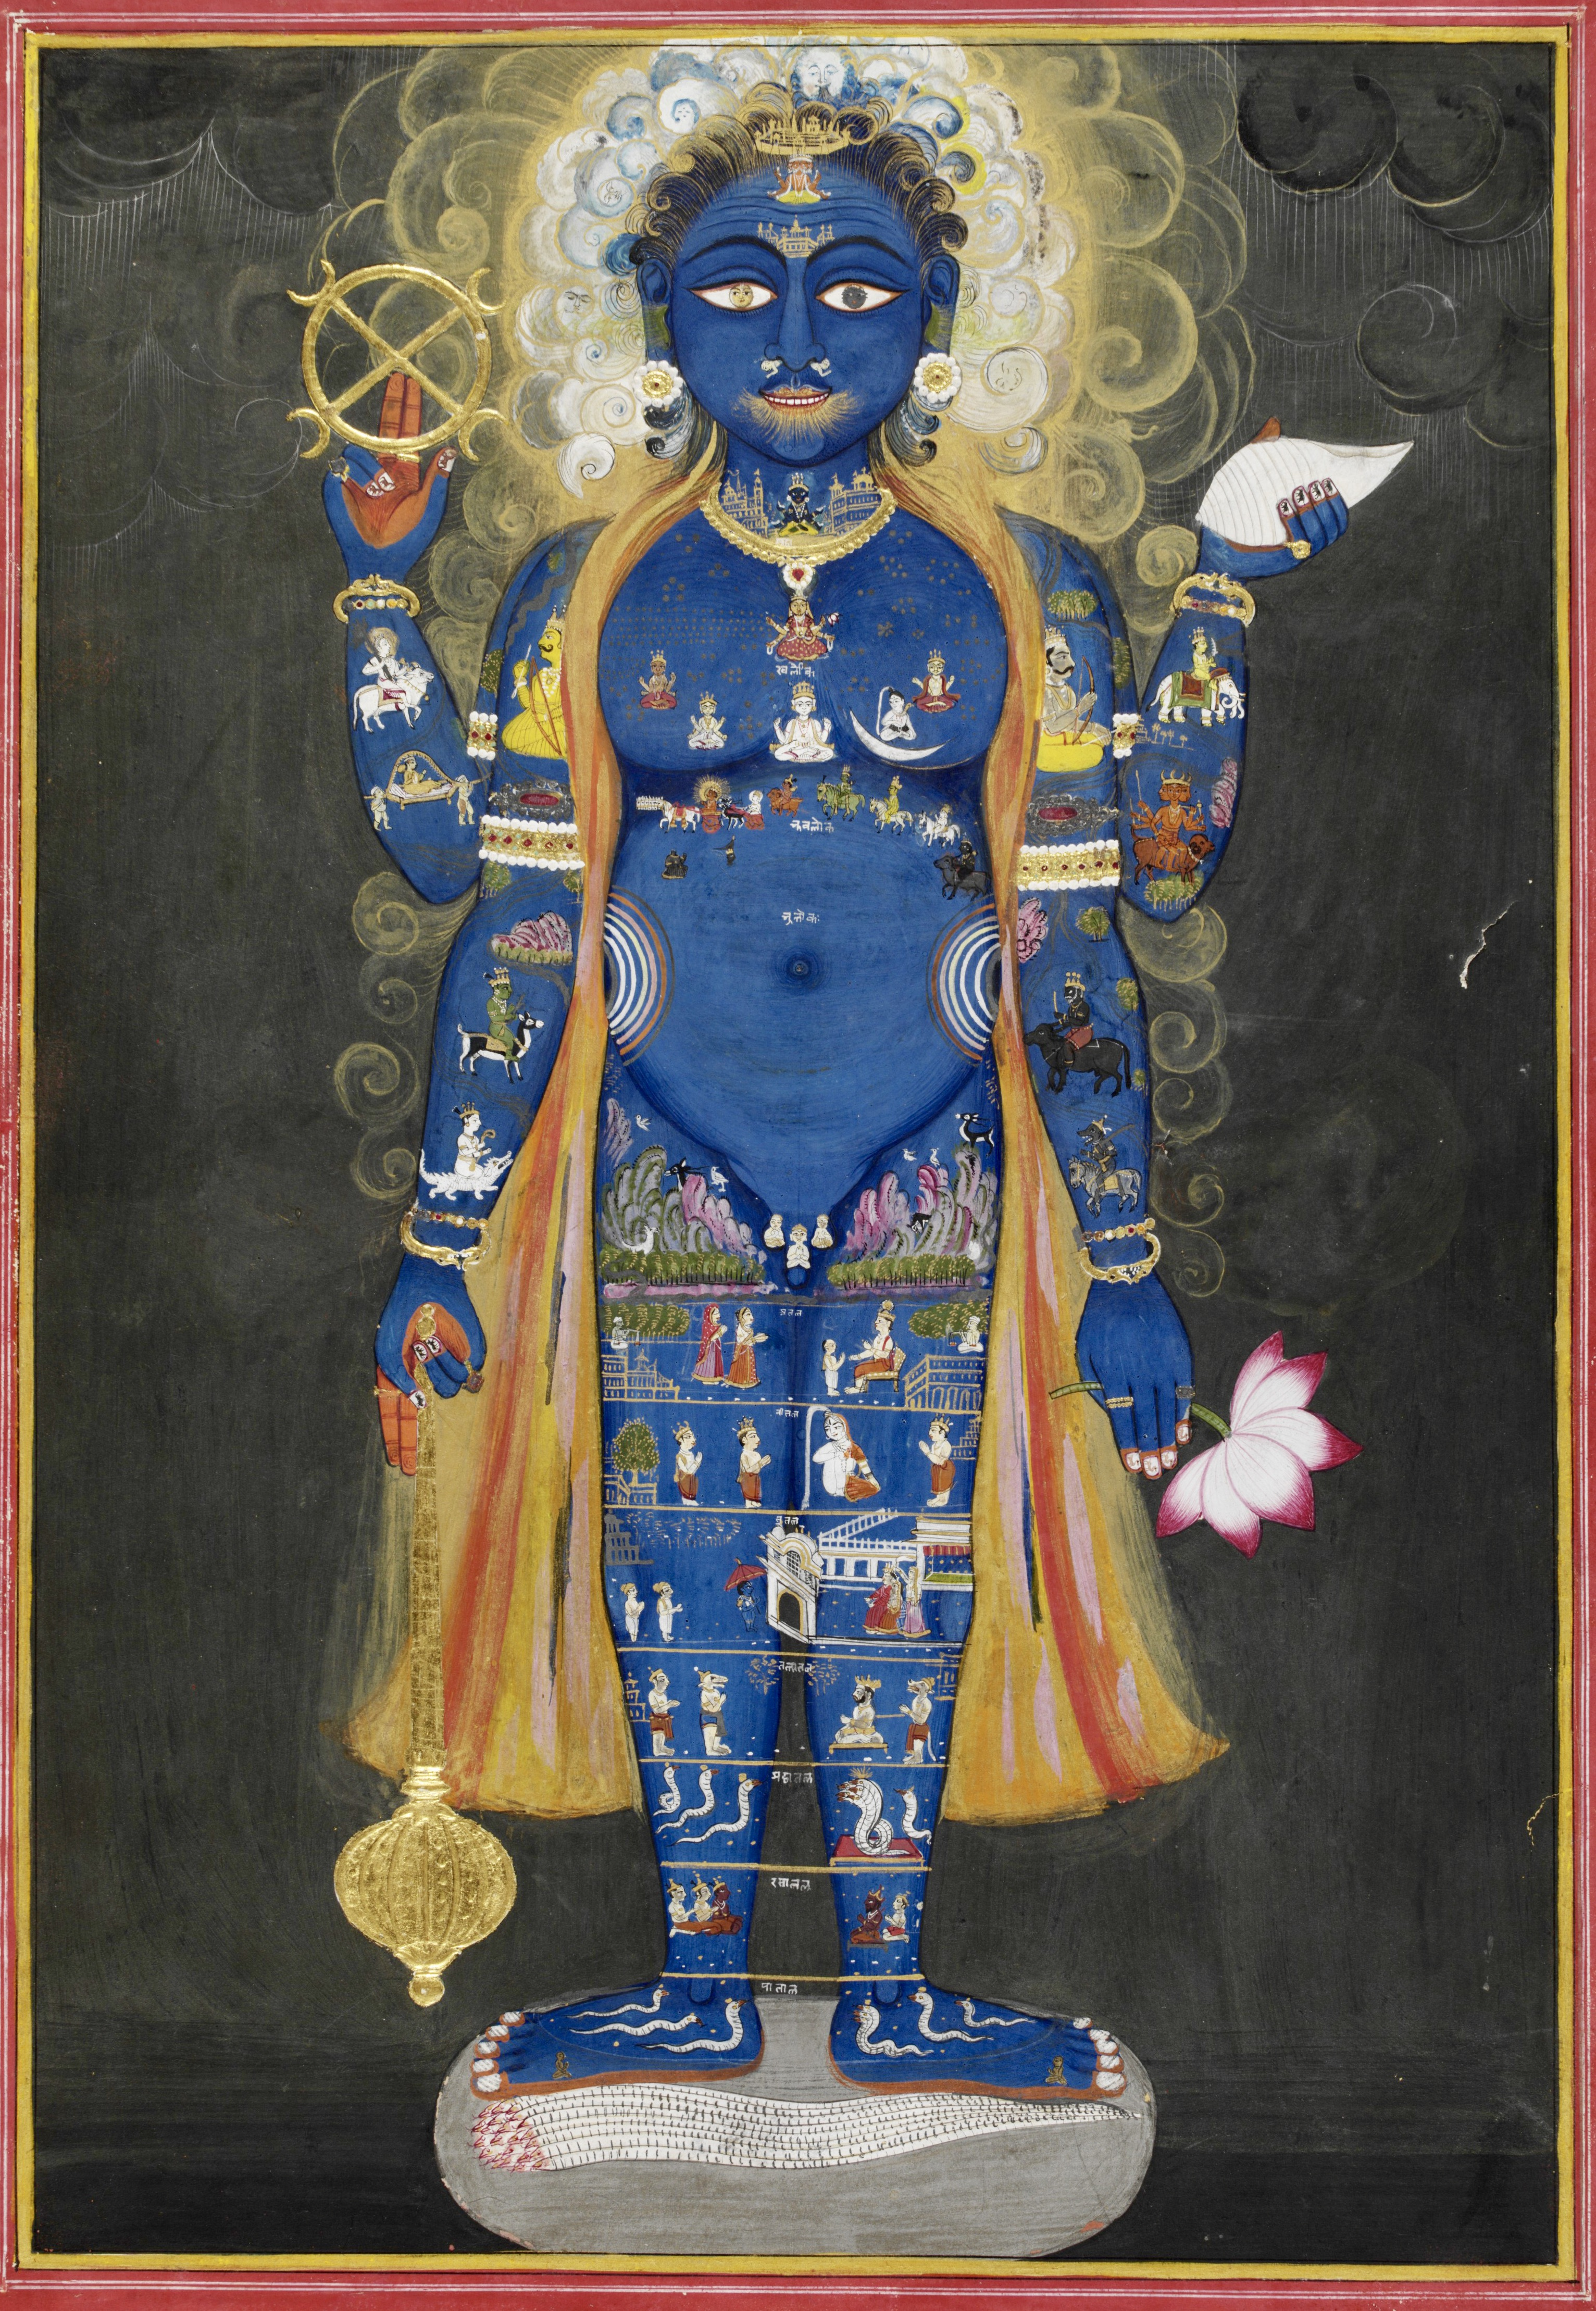
\includegraphics[width=1\textwidth]{pics/Vishnu_Vishvarupa_cropped.jpg}
	\caption{Viṣṇu Viśvarūpa, India, Rajasthan, Jaipur, ca. 1800–1820, Opaque watercolor and gold on paper, 38.5 × 28 cm, Victoria and Albert Museum, London, Given by Mrs. Gerald Clark.}
	\label{fig1}
      \end{figure}
\clearpage
  \begin{figure}[ht]
	\centering
  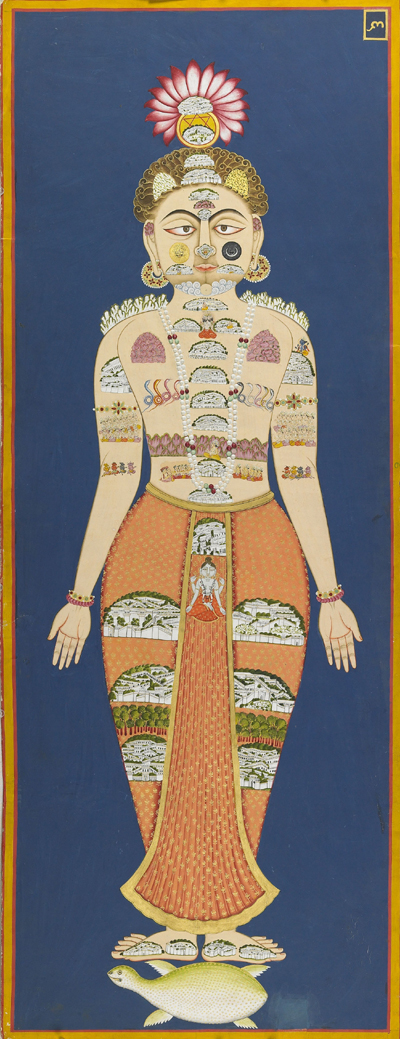
\includegraphics[width=0.5\textwidth]{pics/The_Equivalence_of_Self_and_Universe_(detail),_folio_6_from_the_Siddha_Siddhanta_Paddhati,_(Bulaki),_1824_(Samvat_1881);_122_x_46_cm._Mehrangarh_Museum_Trust..jpg}
	\caption{The Equivalence of Self and Universe (detail), folio 6 from the \textit{Siddhasiddhāntapaddhati} (Bulaki), India, Rajasthan, Jodhpur, 1824 (Samvat 1881), 122 x 46 cm, RJS 2378, Mehragarh Museum Trust.}
	\label{fig2}
      \end{figure}
      % \end{landscape}


\chapter{Bibliography}
 \label{sec:bibli}
   \clearpage
\newpage 
\thispagestyle{empty}
\quad  \addtocounter{page}{-1}

\printbibliography[heading=subbibintoc, title=Consulted Manuscripts, keyword=codex]

\printbibliography[heading=subbibintoc, title=Printed Editions, keyword=printsource]

\printbibliography[heading=subbibintoc, title=Secondary Literature, keyword=seclit]

\printbibliography[heading=subbibintoc, title=Online Sources, keyword=onlinesource]

\end{document}
